\justifying
\section{Introduction}
Today, there is a blossoming of studies on graphene oxide-based membranes (GOMs) for water treatment driven by the simplicity of stacking graphene oxide (GO) monolayers into a laminate structure,\cite{mi2014graphene} which allows the passage of water while retaining larger molecules via size exclusion (Fig.~\ref{Fig1_pap2}a).\cite{nair2012unimpeded} However, a review of the GOM literature reveals a large variability (orders of magnitude) in experimental and simulation water permeability outputs without any quantitative attempt to create a unifying theory, allowing these discrepancies to be ignored.\\
A number of recent investigations have focused on design and construction of GOM heteronanoarchitectures, even though the basic physical phenomena controlling GO assembly are not yet understood. A few studies have hinted at specific GOM water treatment applications, although there is not a clear consensus on whether GOM will be practical for ultra/nanofiltration (NF) or reverse osmosis (RO). The potential number of GO surface chemistry\cite{Dreyer2010} and flake dimension, combinations\cite{amadei2016fabrication} as well as GO metastability,\cite{kim2012room} does not assist in creating a clearer picture. All of these disparities decrease the signal-to-noise ratio (SNR) when examining GOM studies as a whole. In order to invert the trend and increase GOM SNR, we suggest a nomenclature for GOM classification and identify a number of key challenges that should be addressed.

\begin{figure}[h!]
  \centering
  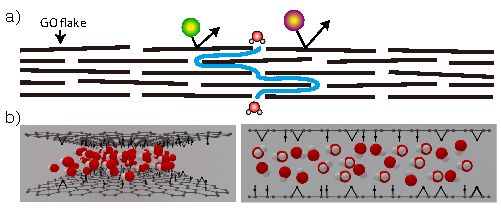
\includegraphics[width=5in]{paper2/Fig1.pdf}
  \caption{\textbf{GOM schematic}. \textbf{(a)} GOM rejection mechanism by size exclusion. \textbf{(b)} 3D (left) and 2D (right) sketch of the water structure in a GOM nanochannel. Note the water hydrogen-bonding interaction with GOM surface oxy-functional groups. Reprinted with permission from ref\cite{montessori2017extended}.}
  \label{Fig1_pap2}
\end{figure}
\section{Results and Discussion}
\subsection{Extreme Variability in Experimental Output}
GOM pure water permeabilities, expressed in LMH-bar (\textit{i.e.}, L m\textsuperscript{-2} h\textsuperscript{-1} bar\textsuperscript{-1}), from a detailed analysis of the current literature is summarized in (Fig.~\ref{Fig2_pap2}a). Of note is the large variability in reported permeability spanning over 2 orders of magnitude. In order to enhance clarity, GOM are divided into five categories: (i) intercalated-GO (I-GO): GOM formed by the intercalation of high aspect-ratio nanostructures in the GO laminate; (ii) as-prepared pristine GO (P-GO): GOM characterized by a surface (or separation) layer of untreated GO; (iii) chemically modified-GO (CM-GO): GOM consisting of a surface (or separation) layer of chemically modified GO (typically reduced, rGO); (iv) layer-by-layer-GO (LbL-GO): GOM formed by a layer-by-layer method where GO is alternatively deposited with a different material; and (v) GO-composite (GOC): GOM obtained by blending of GO with another material (\textit{e.g.}, polymer).
I-GO displays the greatest permeabilities ($10-200$ LMH-bar) due to the widening of the GOM nanochannels (\textit{i.e.}, the spacing between GO layers) by the introduction of high-aspect- ratio nanostructures such as nanotubes or nanorods of various diameter.\cite{goh2015all,chen2016reduced,wang2014graphene,han2015high} On the other hand, GOC exhibit the lowest permeabilities ($0.5-10$ LMH-bar) due to the embedding of GO in a RO matrix (\textit{e.g.}, polyamide) with a low intrinsic permeability.\cite{safarpour2015thin,chae2015graphene} Intermediates are CM-GO ($0.5-70$ LMH-bar) and P-GO ($3-70$ LMH-bar), with CM-GO having a wide range because the chemical GO modification may involve either surface oxy-group reduction decreasing the spacing of the GOM nanochannel spacing or functional group addition increasing the spacing.\cite{Han2013,xia2015ultrathin} LbL-GO ($1-3$ LMH-bar) display lesser permeabilities as compared to those of P-GO ($3-70$ LMH-bar) because LbL has a more ordered laminar structure due to improved intralayer GO packing.\cite{choi2013layer,Hu2013}\\
The proposed categories have a reduced permeability range (typically $20-30$-fold) as compared to the data set as a whole ($\approx400$-fold) and may assist the community in comparing results between GOM studies.
The intrinsic permeability for P-GO, CM-GO, and LbL-GO is displayed in (Fig.~\ref{Fig2_pap2}b). The intrinsic permeability is obtained by multiplying the permeability by the thickness of the GO layer and then normalizing to the greatest value for clarity. Note, I-GO and GOC are not composed of a distinct GO layer; thus, the GO thickness could not be determined (see Table~\ref{tbl1_pap2}). The large variability in the intrinsic permeability data is striking. For example, P-GO intrinsic permeabilities span over 4 orders of magnitude. The CM-GO and LbL-GO values also display a large variability ($>3$ orders of magnitude), which is difficult to explain by varying the reduction technique or LbL process. We identified three possible causes for such a noisy GOM permeability spectrum.
\begin{itemize}
 \item First, although all reports claim to work with GO, the material can vary significantly from one report to another (see details in the GO standardization discussion).
 \item Second, some variability can be attributed to improper membrane performance evaluation as many reported experiments were not run long enough for permeability to reach steady-state (always lower than the initial permeability), that is, several reports evaluate permeability with just a few milliliters (or a few minutes) of water permeation while it can take hours to achieve steady-state. From an environmental engineering perspective, this may also affect rejection (size exclusion) performance that could be confused with adsorption to the high specific surface area GO ($>10^{2}$ m\textsuperscript{2} g\textsuperscript{-1}).\cite{yang2011removal,Graphenea}
 \item Third, GOM may contain large macroscopic defects (basal plane holes; disordered stacking), leading to erroneous conclusions on 1D fast water transport (FWT; similar to carbon nanotubes, CNTs) in the 2D GOM nanochannels (see the fast water transport discussion for details). For instance, GO reduction via thermal annealing under ambient conditions at 150\textdegree C can create basal plane holes $>10$ nm in diameter.\cite{qiu2011controllable}
\end{itemize}
\begin{figure}
  \centering
  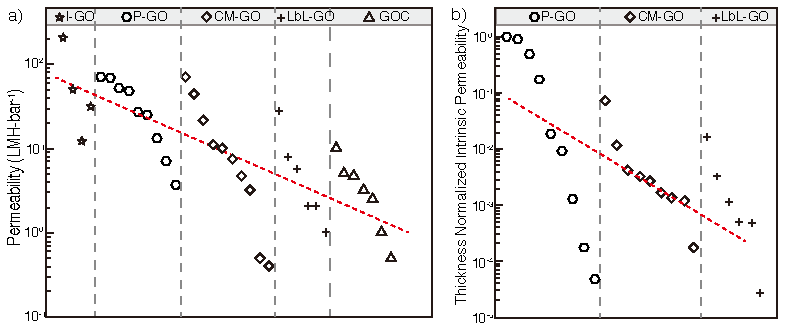
\includegraphics[width=6in]{paper2/Fig2.pdf}
  \caption{\textbf{GOM pure water permeability}. \textbf{(a)} GOM permeability expressed in LMH-bar for all five categories in descending order. The dashed line represents the linear decrease in the average permeability from I-GO to GOC. \textbf{(b)} Normalized intrinsic permeability for the three relevant categories.}
  \label{Fig2_pap2}
\end{figure}

\begin{table}
 \begin{center}
 \caption{\textbf{GOM Pure Water Permeability and GO Properties.}}
  \label{tbl1_pap2}
  \begin{tabular}{*7c}
        Category &  $\#$ & Permeability   & Thickness & Oxidation & Note & Ref.\\
         &  & (LMH-bar)  & (nm) &  & & \\
        \hline
        I-GO & 1 & 205  & n/a & n/a & intercalation with carbon dots & \cite{wang2014graphene}\\
        I-GO & 2 & 50 & n/a & n/a & intercalation with CNT & \cite{goh2015all}\\
        I-GO & 3 & 12.13  & n/a & n/a & intercalation with CNT & \cite{han2015high}\\
        I-GO & 3 & 31.5 & n/a & n/a & intercalation with CNT & \cite{chen2016reduced}\\
        \hline
        P-GO & 5 & 71 & 2000 & n/a & modified Hummers\textquotesingle \, method & \cite{huang2013salt}\\
        P-GO & 6 & 70 & 1000 & 53.7\% (C-O, C=O) & modified \textquotesingle \, method & \cite{ying2014plane}\\
         &  &  &  & 46.3\% (C-C, C=C) &  & \\
        P-GO & 7 & 53 & 2500 & n/a & modified Hummers\textquotesingle \, method & \cite{wang2014graphene}\\
        P-GO & 8 & 48 & 55 & n/a & modified Hummers\textquotesingle \, method & \cite{goh2015all}\\
        P-GO & 9 & 27.2 & 50 & 45.8\% (C-O, C=O) & commercial & \cite{xia2015ultrathin}\\
        &  &  &  & 54.2\% (C-C, C=C) &  & \\
        P-GO & 10 & 25 & 1 & n/a & modified Hummers\textquotesingle \, method & \cite{goh2015graphene}\\
         & 10 & & & & and Offeman's method & \\
        P-GO & 11 & 212.9 & 2000 & n/a & modified Hummers\textquotesingle \, method & \cite{huang2013salt}\\
        P-GO & 12 & 7 & 1 & n/a & modified Hummers\textquotesingle \, method & \cite{goh2015graphene}\\
         & 10 & & & & and Offema's method & \\
        P-GO & 13 & 3.75 & 50 & 53.7\% (C-O, C=O)& modified Hummers\textquotesingle \, method & \cite{amadei2017role}\\
         &  &  &  & 31.4\% (C-C, C=C) &  & \\
        \hline
        CM-GO & 14 & 71 & 150 & n/a & GO reduced with hydrazine & \cite{akbari2016large}\\
        CM-GO & 15 & 45 &  n/a & n/a & GO reduced with thermal & \cite{qiu2011controllable}\\
         & & &  &  & annealing in air & \\
        CM-GO & 16 & 12.8 &  22 & n/a & GO reduced with base reflux & \cite{han2013ultrathin}\\
        CM-GO & 17 & 11 &  55 & n/a & GO reduced with hydroiodic acid & \cite{goh2015all}\\
        CM-GO & 18 & 10 &  170 & n/a & GO reduced with hydrazine & \\
        CM-GO & 19 & 7.5 &  50 & 20.1\% (C-O, C=O) & GO functionalized/reduced & \cite{xia2015ultrathin}\\
         & &  &  & 59.9\% (C-C, C=C) & with diamine & \\
        CM-GO & 20 & 4.76 &  40 & n/a &  GO reduced with thermal & \cite{han2015high}\\
        & & &  &  & annealing in solution & \\
        CM-GO & 21 & 3.26 & 53 & n/a &  GO reduced with base reflux  & \cite{han2013ultrathin}\\
        CM-GO & 22 & 0.5 & 50 & 76.5\% (C-O, C=O) &  GO reduced with hydroiodic acid  & \cite{amadei2017role}\\
        & &  &  & 24.5\% (C-C, C=C) &  & \\
        CM-GO & 23 & 0.4 & 600 & n/a &  GO reduced with ascorbic acid  & \cite{chen2016reduced}\\
        \hline
        LbL-GO & 24 & 27.6 & 87 & 60\% (C-O, C=O) &  GO cross-linked by  & \cite{Hu2013}\\
        & &  &  & 50\% (C-C, C=C) & benzenetricarbonyl trichloride & \\
        LbL-GO & 25 & 8 & 8.7 & 60\% (C-O, C=O) &  GO cross-linked by  & \cite{Hu2013}\\
        & &  &  & 40\% (C-C, C=C) & benzenetricarbonyl trichloride & \\
        LbL-GO & 26 & 5.8 & 82.5 & O/C=25-28\% &  GO cross-linked by  & \cite{hu2014layer}\\
        & &  &  &  & poly(allylaminehydrochloride)& \\
        LbL-GO & 27 & 2.1 & 33 & O/C=30-50\% &  GO cross-linked by  & \cite{hu2014layer}\\
        & &  &  &  & poly(allylaminehydrochloride)& \\
        \end{tabular}
    \end{center}
\end{table}

\begin{table}[t!]
 \begin{center}
  \begin{tabular}{*7c}
        Category &  $\#$ & Permeability   & Thickness & Oxidation & Note & Ref.\\
         &  & (LMH-bar)  & (nm) &  & & \\
        \hline
        LbL-GO & 28 & 2 & 80 & O/C=50\% &  GO cross-linked by  & \cite{hu2014layer}\\
        & &  &  &  & poly(allylaminehydrochloride)& \\
        LbL-GO & 29 & 1 & 4 & na &  Lbl structure  & \cite{choi2013layer}\\
        \hline
        GOC-GO & 30 & 10 & n/a & na &  GO mixed with polyaniline  & \cite{akin2014green}\\
        GOC-GO & 31 & 5 & n/a & na &  GO mixed with polysulfone & \cite{ganesh2013enhanced}\\
        GOC-GO & 32 & 4.7 & n/a & na &  GO mixed with polysulfone & \cite{ganesh2013enhanced}\\
        GOC-GO & 33 & 3.2 & n/a & na &  GO mixed with titanium dioxide & \cite{safarpour2015thin}\\
        GOC-GO & 34 & 2.5 & n/a & na &  GO mixed with polyaniline  & \cite{akin2014green}\\
        GOC-GO & 35 & 1 & n/a & 65\% (C-C, C=C) &  GO mixed with polyamide  & \cite{chae2015graphene}\\
         & &  &  & 35\% (C-C, C=C) & & \\
        GOC-GO & 36 & 0.5 & n/a & 65\% (C-C, C=C) &  GO mixed with & \cite{zinadini2014preparation}\\
         & &  &  &  & poly(ethersulfone)& \\
        \end{tabular}
    \end{center}
\end{table}
\newpage
\begin{comment}
\begin{longtable}[t!]{|ccccccc|}
\caption{\textbf{GOM Pure Water Permeability and GO Properties.}In each category, the permeability is listed highest to lowest.}  \label{tbl1_pap2} \\

\hline \multicolumn{1}{|c|}{Cat/} & \multicolumn{1}{c|}{ $\#$} & \multicolumn{1}{c|}{Perm. (LMH-bar)}&
\multicolumn{1}{c|}{Thick. (nm}&
\multicolumn{1}{c|}{GO Oxidation}&
\multicolumn{1}{c|}{Note}&
\multicolumn{1}{c|}{Ref.}\\
\endfirsthead


\multicolumn{7}{c}%
{{\bfseries \tablename\ \thetable{} -- continued from previous page}} \\
\hline\multicolumn{1}{|c|}{Cat.} & 
\multicolumn{1}{c|}{ $\#$} & \multicolumn{1}{c|}{Perm. (LMH-bar)}&
\multicolumn{1}{c|}{Thick. (nm)}&
\multicolumn{1}{c|}{GO Oxidation}&
\multicolumn{1}{c|}{Note}&
\multicolumn{1}{c|}{Ref.}\\
&  &(LMH-bar) & (nm) &  &  &
\endhead


\hline \multicolumn{7}{|r|}{{Continued on next page.}} \\ \hline
\endfoot

\hline \hline
\endlastfoot
        \hline
        I-GO & 1 & 205  & n/a & n/a & intercalation with carbon dots & \cite{wang2014graphene}\\
        I-GO & 2 & 50 & n/a & n/a & intercalation with CNT & \cite{goh2015all}\\
        I-GO & 3 & 12.13  & n/a & n/a & intercalation with CNT & \cite{han2015high}\\
        I-GO & 3 & 31.5 & n/a & n/a & intercalation with CNT & \cite{chen2016reduced}\\
        \hline
        P-GO & 5 & 71 & 2000 & n/a & modified Hummers\textquotesingle \, method & \cite{huang2013salt}\\
        P-GO & 6 & 70 & 1000 & 53.7\% (C-O, C=O) & modified \textquotesingle \, method & \cite{ying2014plane}\\
         &  &  &  & 46.3\% (C-C, C=C) &  & \\
        P-GO & 7 & 53 & 2500 & n/a & modified Hummers\textquotesingle \, method & \cite{wang2014graphene}\\
        P-GO & 8 & 48 & 55 & n/a & modified Hummers\textquotesingle \, method & \cite{goh2015all}\\
        P-GO & 9 & 27.2 & 50 & 45.8\% (C-O, C=O) & commercial & \cite{xia2015ultrathin}\\
        &  &  &  & 54.2\% (C-C, C=C) &  & \\
        P-GO & 10 & 25 & 1 & n/a & modified Hummers\textquotesingle \, method & \cite{goh2015graphene}\\
         & 10 & & & & and Offeman's method & \\
        P-GO & 11 & 212.9 & 2000 & n/a & modified Hummers\textquotesingle \, method & \cite{huang2013salt}\\
        P-GO & 12 & 7 & 1 & n/a & modified Hummers\textquotesingle \, method & \cite{goh2015graphene}\\
         & 10 & & & & and Offeman's method & \\
        P-GO & 13 & 3.75 & 50 & 53.7\% (C-O, C=O)& modified Hummers\textquotesingle \, method & \cite{amadei2017role}\\
         &  &  &  & 31.4\% (C-C, C=C) &  & \\
        \hline
        CM-GO & 14 & 71 & 150 & n/a & GO reduced with hydrazine & \cite{akbari2016large}\\
        CM-GO & 15 & 45 &  n/a & n/a & GO reduced with thermal & \cite{qiu2011controllable}\\
         & & &  &  & annealing in air & \\
        CM-GO & 16 & 12.8 &  22 & n/a & GO reduced with base reflux & \cite{han2013ultrathin}\\
        CM-GO & 17 & 11 &  55 & n/a & GO reduced with hydroiodic acid & \cite{goh2015all}\\
        CM-GO & 18 & 10 &  170 & n/a & GO reduced with hydrazine & \\
        CM-GO & 19 & 7.5 &  50 & 20.1\% (C-O, C=O) & GO functionalized/reduced & \cite{xia2015ultrathin}\\
         & &  &  & 59.9\% (C-C, C=C) & with diamine & \\
        CM-GO & 20 & 4.76 &  40 & n/a &  GO reduced with thermal & \cite{han2015high}\\
        & & &  &  & annealing in solution & \\
        CM-GO & 21 & 3.26 & 53 & n/a &  GO reduced with base reflux  & \cite{han2013ultrathin}\\
        CM-GO & 22 & 0.5 & 50 & 76.5\% (C-O, C=O) &  GO reduced with hydroiodic acid  & \cite{amadei2017role}\\
        & &  &  & 24.5\% (C-C, C=C) &  & \\
        CM-GO & 23 & 0.4 & 600 & n/a &  GO reduced with ascorbic acid  & \cite{chen2016reduced}\\
        \hline
        LbL-GO & 24 & 27.6 & 87 & 60\% (C-O, C=O) &  GO cross-linked by  & \cite{Hu2013}\\
        & &  &  & 50\% (C-C, C=C) & benzenetricarbonyl trichloride & \\
        LbL-GO & 25 & 8 & 8.7 & 60\% (C-O, C=O) &  GO cross-linked by  & \cite{Hu2013}\\
        & &  &  & 40\% (C-C, C=C) & benzenetricarbonyl trichloride & \\
        LbL-GO & 26 & 5.8 & 82.5 & O/C=25-28\% &  GO cross-linked by  & \cite{hu2014layer}\\
        & &  &  &  & poly(allylaminehydrochloride)& \\
        LbL-GO & 27 & 2.1 & 33 & O/C=30-50\% &  GO cross-linked by  & \cite{hu2014layer}\\
        & &  &  &  & poly(allylaminehydrochloride)& \\
        LbL-GO & 28 & 2 & 80 & O/C=50\% &  GO cross-linked by  & \cite{hu2014layer}\\
        & &  &  &  & poly(allylaminehydrochloride)& \\
        LbL-GO & 29 & 1 & 4 & na &  Lbl structure  & \cite{choi2013layer}\\
        \hline
        GOC-GO & 30 & 10 & n/a & na &  GO mixed with polyaniline  & \cite{akin2014green}\\
        GOC-GO & 31 & 5 & n/a & na &  GO mixed with polysulfone & \cite{ganesh2013enhanced}\\
        GOC-GO & 32 & 4.7 & n/a & na &  GO mixed with polysulfone & \cite{ganesh2013enhanced}\\
        GOC-GO & 33 & 3.2 & n/a & na &  GO mixed with titanium dioxide & \cite{safarpour2015thin}\\
        GOC-GO & 34 & 2.5 & n/a & na &  GO mixed with polyaniline  & \cite{akin2014green}\\
        GOC-GO & 35 & 1 & n/a & 65\% (C-C, C=C) &  GO mixed with polyamide  & \cite{chae2015graphene}\\
         & &  &  & 35\% (C-C, C=C) & & \\
        GOC-GO & 36 & 0.5 & n/a & 65\% (C-C, C=C) &  GO mixed with & \cite{zinadini2014preparation}\\
         & &  &  &  & poly(ethersulfone)& \\
\end{longtable}

\begin{center}
\begin{longtable}{|l|l|l|}
\caption{A sample long table.} \label{tab:long} \\

\hline \multicolumn{1}{|c|}{\textbf{First column}} & \multicolumn{1}{c|}{\textbf{Second column}} & \multicolumn{1}{c|}{\textbf{Third column}} \\ \hline 
\endfirsthead

\multicolumn{3}{c}%
{{\bfseries \tablename\ \thetable{} -- continued from previous page}} \\
\hline \multicolumn{1}{|c|}{\textbf{First column}} & \multicolumn{1}{c|}{\textbf{Second column}} & \multicolumn{1}{c|}{\textbf{Third column}} \\ \hline 
\endhead

\hline \multicolumn{3}{|r|}{{Continued on next page}} \\ \hline
\endfoot

\hline \hline
\endlastfoot
One & abcdef ghjijklmn & 123.456778 \\
One & abcdef ghjijklmn & 123.456778 \\
One & abcdef ghjijklmn & 123.456778 \\
One & abcdef ghjijklmn & 123.456778 \\
One & abcdef ghjijklmn & 123.456778 \\
One & abcdef ghjijklmn & 123.456778 \\
One & abcdef ghjijklmn & 123.456778 \\
One & abcdef ghjijklmn & 123.456778 \\
One & abcdef ghjijklmn & 123.456778 \\
One & abcdef ghjijklmn & 123.456778 \\
One & abcdef ghjijklmn & 123.456778 \\
One & abcdef ghjijklmn & 123.456778 \\
One & abcdef ghjijklmn & 123.456778 \\
One & abcdef ghjijklmn & 123.456778 \\
One & abcdef ghjijklmn & 123.456778 \\
One & abcdef ghjijklmn & 123.456778 \\
One & abcdef ghjijklmn & 123.456778 \\
One & abcdef ghjijklmn & 123.456778 \\
One & abcdef ghjijklmn & 123.456778 \\
One & abcdef ghjijklmn & 123.456778 \\
One & abcdef ghjijklmn & 123.456778 \\
One & abcdef ghjijklmn & 123.456778 \\
One & abcdef ghjijklmn & 123.456778 \\
One & abcdef ghjijklmn & 123.456778 \\
One & abcdef ghjijklmn & 123.456778 \\
One & abcdef ghjijklmn & 123.456778 \\
One & abcdef ghjijklmn & 123.456778 \\
One & abcdef ghjijklmn & 123.456778 \\
One & abcdef ghjijklmn & 123.456778 \\
One & abcdef ghjijklmn & 123.456778 \\
One & abcdef ghjijklmn & 123.456778 \\
One & abcdef ghjijklmn & 123.456778 \\
One & abcdef ghjijklmn & 123.456778 \\
One & abcdef ghjijklmn & 123.456778 \\
One & abcdef ghjijklmn & 123.456778 \\
One & abcdef ghjijklmn & 123.456778 \\
One & abcdef ghjijklmn & 123.456778 \\
One & abcdef ghjijklmn & 123.456778 \\
One & abcdef ghjijklmn & 123.456778 \\
One & abcdef ghjijklmn & 123.456778 \\
One & abcdef ghjijklmn & 123.456778 \\
One & abcdef ghjijklmn & 123.456778 \\
One & abcdef ghjijklmn & 123.456778 \\
One & abcdef ghjijklmn & 123.456778 \\
One & abcdef ghjijklmn & 123.456778 \\
One & abcdef ghjijklmn & 123.456778 \\
One & abcdef ghjijklmn & 123.456778 \\
One & abcdef ghjijklmn & 123.456778 \\
One & abcdef ghjijklmn & 123.456778 \\
One & abcdef ghjijklmn & 123.456778 \\
One & abcdef ghjijklmn & 123.456778 \\
One & abcdef ghjijklmn & 123.456778 \\
One & abcdef ghjijklmn & 123.456778 \\
One & abcdef ghjijklmn & 123.456778 \\
One & abcdef ghjijklmn & 123.456778 \\
One & abcdef ghjijklmn & 123.456778 \\
One & abcdef ghjijklmn & 123.456778 \\
One & abcdef ghjijklmn & 123.456778 \\
One & abcdef ghjijklmn & 123.456778 \\
One & abcdef ghjijklmn & 123.456778 \\
One & abcdef ghjijklmn & 123.456778 \\
One & abcdef ghjijklmn & 123.456778 \\
One & abcdef ghjijklmn & 123.456778 \\
One & abcdef ghjijklmn & 123.456778 \\
One & abcdef ghjijklmn & 123.456778 \\
One & abcdef ghjijklmn & 123.456778 \\
One & abcdef ghjijklmn & 123.456778 \\
One & abcdef ghjijklmn & 123.456778 \\
One & abcdef ghjijklmn & 123.456778 \\
One & abcdef ghjijklmn & 123.456778 \\
One & abcdef ghjijklmn & 123.456778 \\
One & abcdef ghjijklmn & 123.456778 \\
One & abcdef ghjijklmn & 123.456778 \\
One & abcdef ghjijklmn & 123.456778 \\
One & abcdef ghjijklmn & 123.456778 \\
One & abcdef ghjijklmn & 123.456778 \\
One & abcdef ghjijklmn & 123.456778 \\
One & abcdef ghjijklmn & 123.456778 \\
One & abcdef ghjijklmn & 123.456778 \\
One & abcdef ghjijklmn & 123.456778 \\
\end{longtable}
\end{center}
\end{comment}
\newpage
\subsection{Need for Standardization and Lack of in Situ Characterization}
For pristine graphene research, standardization is underway. The International Electrotechnical Commission (IEC) released the IEC 62565-3-1,\cite{IEC} which aims to tabulate all relevant graphene properties and standardized protocols for characterization. The end goal is to enable the purchase of materials with very similar properties and drive the broad use of graphene in manufacturing and industry. Concurrently, Graphene Flagship is establishing a standardization committee with the aim of creating a database listing all of the various graphene forms, their properties, and methods to characterize those properties.\cite{Flag} A similar standardization is necessary for GO in order to enable successful commercialization and industrial application of the material. However, from our experience, as well as from discussions with academics and GO producers, we are still far from a standardized GO product. For example, characterization of GO from various producers yielded widely ranging material chemistry, as noted in Table ~\ref{tbl1_pap2}, where the GO oxidation is characterized in less than one-third of the studies and that reported has a wide range of oxygen content.\\
In general, 2D material properties can be intrinsically divided into morphology and chemistry, which in turn affects practical properties such as electrical, mechanical, thermal, magnetic, and optical functionality.\\
GO morphology can be easily characterized by drop-casting a dilute solution of GO ($\approx10^{-3}$ wt\%) onto a flat substrate (\textit{i.e.}, silicon chip) and performing scanning electron microscope (SEM) imaging (Fig.~\ref{Fig3_pap2}a left) and subsequent thorough image analysis (Fig.~\ref{Fig3_pap2}a right). From SEM image analysis, the GO flake size distribution and monolayer percentage (flake contrast) can be determined,\cite{hernandez2008high} which can be utilized for standardization. Although atomic force microscopy (AFM) can also be used to evaluate GO morphology, it has lower throughput compared to SEM (10s $\mu$m\textsuperscript{2}s\textsuperscript{-1} compared to 1000s $\mu$m\textsuperscript{2}s\textsuperscript{-1}), and AFM thickness results can be affected by the AFM operation mode and the level of humidity.\cite{santos2012effects}

\begin{figure}[h!]
  \centering
  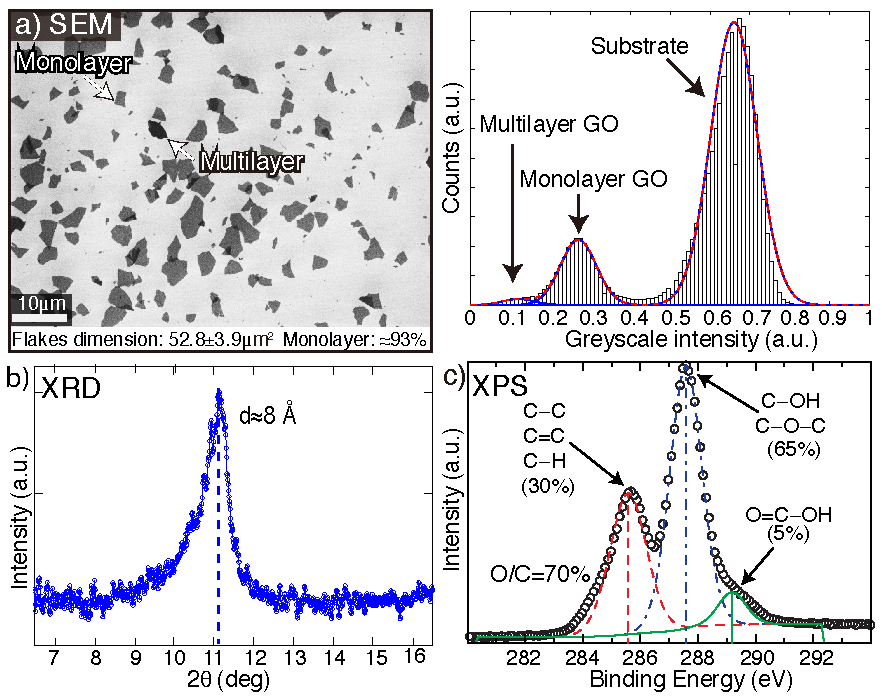
\includegraphics[width=5in]{paper2/Fig3.pdf}
  \caption{\textbf{GO chemistry and morphology characterization.}. \textbf{(a)} GO morphology analyzed by SEM. The histogram summarizes the gray scale intensity counts of the SEM image, which can be deconvoluted with three Gaussian distributions whose areas represent the substrate, GO monolayer, and GO multilayer fractions. \textbf{(b)} XRD spectra of multilayer GO where d is the GO nanochannel spacing. \textbf{(c)} Integration of the XPS C1s spectra deconvolution to quantify GO carbon bonding. Reproduced from ref. \cite{amadei2016fabrication}.
 relevant categories.}
  \label{Fig3_pap2}
\end{figure}
Because GO flakes tend to stack in a laminar fashion, X-ray diffraction (XRD) is recommended to evaluate GOM nanochannel spacing (Fig.~\ref{Fig3_pap2}b). From spacing information, it may be possible to infer the GOM molecular weight cutoff (\textit{i.e.}, rejection performance), making XRD a paramount tool for GOM characterization. Although GOM spacing has been reported,\cite{xia2015ultrathin,talyzin2014structure} there is a lack of in situ characterization techniques. In particular, the evaluation of GOM spacing while the membrane is under operation has not been reported as it would require performing XRD analysis while pressurized water is flowing through the GOM. To date, XRD data in the literature refers to either the ''dry'' or ''wet'' state, qualitatively reporting GOM swelling (up to 25\%) when immersed in water.\cite{talyzin2014structure} However, these characterizations will not resemble the status of GOM under operation and may neglect other physical phenomena such as pressure-induced GO flake rearrangement and/or the presence of adsorbed molecules (spacers).\\
A proper GOM morphology characterization (GO flake dimension spacing) may also provide information on GOM tortuosity. The high GO flake aspect ratio can yield a membrane tortuosity that negates the benefit of an ultrathin ($<100$ nm) membrane. Although considered an important membrane property, GOM tortuosity has not yet been considered in depth. If not single-layer GO, then for every additional GO layer there will be an additional water nanochannel. In turn, the water permeate will roughly travel on average half of the GO flake length for every additional layer. Thus, neglecting the presence of defects, for a bilayer GOM with 10 $\mu$m flakes, the water will have to travel 5 $\mu$m, which is significantly greater ($1000$-fold) than the 5 nm thickness.\\
GO chemistry can be quantitatively analyzed by X-ray photoelectron spectroscopy (XPS), providing information on the oxygen and/or specific functional group content, which directly affects practical properties (\textit{e.g.}, spacing and conductivity).\cite{mattevi2009evolution} Deconvolution of the XPS C1s spectrum (Fig.~\ref{Fig3_pap2}c) can be used to quantify the predominant carbon bond type, in accordance with the Lerf-Klinowski model:\cite{lerf1998structure} (i) single (C-C) and double (C=C) carbon-carbon bonds; (ii) epoxide (C-O-C) and hydroxide (C-OH) single carbon-oxygen bonds; and (iii) carboxylate (O=C-OH) double carbon-oxygen bonds. Further deconvolution aiming to distinguish between epoxide and hydroxide functional groups has to be taken with a grain of salt due to binding energy chemical shifts approaching tool resolution.\cite{wepasnick2011surface}
Raman spectroscopy has also been employed to analyze GO chemistry and generally displays a D band (A\textsubscript{1g} symmetry) at $\approx1350$ cm\textsuperscript{-1} representative of defects/disorder in the basal plane and a G band (E\textsubscript{2g} symmetry) at $\approx1590$ cm\textsuperscript{-1} that corresponds to the in-plane sp\textsuperscript{2} bond stretching.\cite{amadei2014time} However, GO is a metastable material, and the laser irradiation during Raman spectroscopy can unintentionally modify the material, leading to unreliable results.\cite{rogala2016observer} Depending on the acquisition time, this phenomenon also holds for XPS characterization, though with a limited negative effect compared to Raman. Thus, when reporting characterization methods, it is important to specify the acquisition time and other parameters that could alter material properties.\\
GO metastability not only affects the outcomes of characterization techniques but it is also a relevant element to consider when designing a GOM. A clear example is GO photo-reduction/oxidation that is highly dependent on light conditions and the environmental medium.\cite{hou2015photochemical} Thus, it is important to work with either a stable GO material and/or a controlled environment to ensure that GO redox activity, as well as other potential chemistry, is negligible such that properties/performance do not significantly alter with time.\cite{yeh2015origin}

\subsection{Possibility of CNT Fast Water Transport in Graphene Oxide Membrane}
Several studies have reported FWT in GOMs possibly due to the low wall friction experienced by water when traveling through regions of 2D pristine graphene capillaries. At first glance, this could be similar to FWT through 1D CNTs due to a linear water dipole orientation parallel to the CNT axis offering the lowest water-CNT interaction potential.\cite{zuo2009transport,holt2006fast} However, in GOMs, water can move in two directions; thus, the dipole orientation phenomena will not be as significant as that in 1D CNTs as there will be a viscous water-water interaction in one direction perpendicular to the flow. Moreover, due to the H-bonding interaction between water and GO basal plane oxy-groups, ''friction'' will occur when water travels through GO nanochannels; thus, a slip condition seems improbable. This phenomenon is supported by experiments reporting permeability reduction with an increasing GOM thickness indicating Darcy (no-slip) behavior.\cite{chen2016reduced} This experimental evidence clashes with frictionless GOM FWT, which should be independent from permeate path length.\\
However, there are experimental and simulation studies reporting GOM water permeabilities not in accordance with the no-slip condition.\cite{han2013ultrathin} A possible explanation for observation of enhanced permeabilities may be related to the presence of holes and/or macroscopic defects in GOMs, reducing tortuosity and increasing water permeability. Due to the high anisotropy of the GO flake dimension, the effect of GOM defects on the water permeability requires large simulation domains, which are computationally costly with tools currently used to evaluate GOM performance (\textit{i.e.}, molecular dynamics (MD), Fig.~\ref{Fig4_pap2}a-c). Thus, mesoscale simulation tools may offer the opportunity to investigate larger domains and evaluate the effect of GOM defects and tortuosity on water permeability. For example, 2D mesoscale simulations (Fig.~\ref{Fig4_pap2}d-e) recently displayed the potential to model water transport in GOMs and other 2D materials.\cite{montessori2017extended}
Although discussion of GOM water permeability is paramount, selectivity is just as important. For instance, in terms of industrial/municipal applications, a 300\% increase in membrane permeability will decrease the operational energy requirements for a desalination plant by only 2\%; thus, the gain is only in the decrease of capital cost that is a fraction of the overall cost.\cite{werber2016materials}
\begin{figure}[t!]
  \centering
  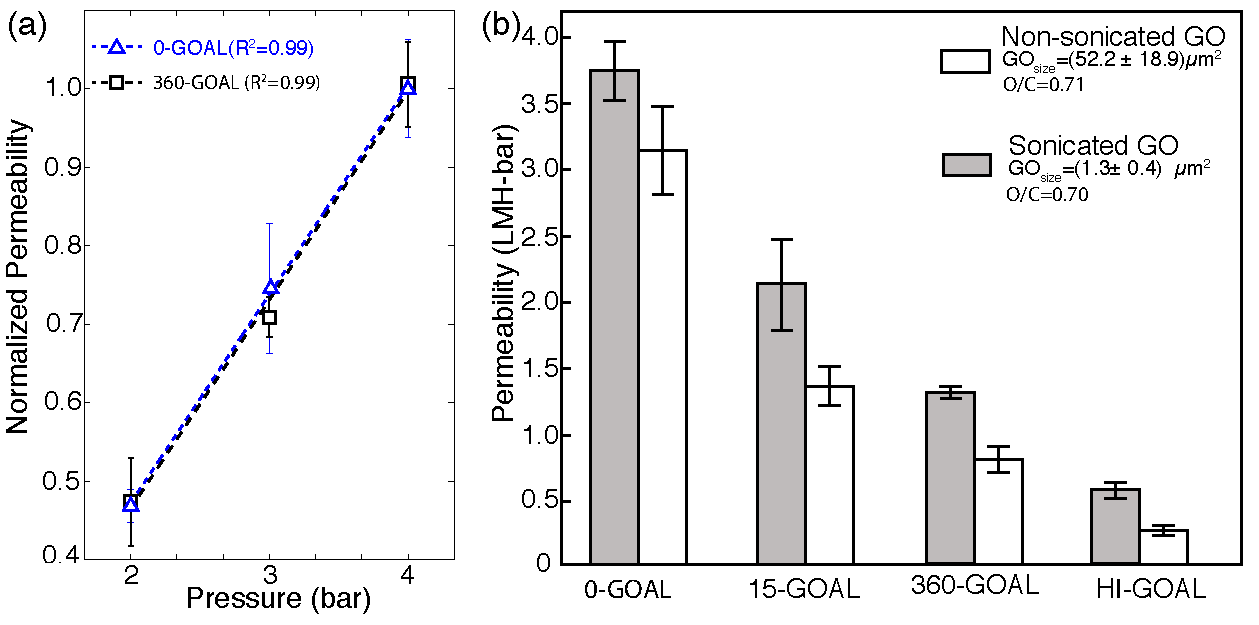
\includegraphics[width=5in]{paper2/Fig4.pdf}
  \caption{\textbf{Simulation of water flow transport within GOMs.}. \textbf{(a-c)} MD simulations of water flow within GOM nanochannels (the scale bar is 2 nm for (c)); reprinted (adapted) with permission from Ref. \cite{wei2014understanding}. \textbf{(d,e)} Mesoscale simulations of water flow inside of GOM nanochannels. The scale bar is 5 nm for (d).}
  \label{Fig4_pap2}
\end{figure}
\subsection{Casting Challenge (Scale-up) and Substrate Paradigm}
For GOMs to succeed in existing laboratories and be employed for industrial applications such as municipal water treatment, they will have to overcome the ''casting'' challenge. So far, three general approaches have been used to cast GO on a support: filtration, casting/coating, and LbL assembly. Filtration onto a porous membrane separates the GO flakes from the solvent, and the filtration force dictates the GOM laminar structure.\cite{hung2014pressure,tsou2015effect} Casting/coating approaches include spray-coating, drop-casting, spin-coating, and doctor blade-casting,\cite{nair2012unimpeded,hongfei2015transparent} and although the latter seems to be a promising casting method for industrial applications,\cite{akbari2016large} it requires GO pretreatment in order to obtain a gel with proper viscous properties and it is unknown how the process affects assembly. The LbL assembly approach is specifically designed to introduce cross-linkers into the GO laminate unless GO is utilized for all layers. The first two methods are highly scalable but suffer from minimal control of GO assembly and final structure. In contrast, the LbL method yields increased control of the GO layer number, packing, and thickness but is characterized by slow throughput, in particular, if the more controlled Langmuir-Blodgett (LB) method is used.\cite{Kim2010} Thus, academic researchers will need to investigate alternatives to traditional casting techniques and/or develop a hybrid approach that can guarantee control of the GO assembly, industrial-scalability, and rapid throughput.\\
A possible hybrid approach is presented in Fig.~\ref{Fig5_pap2}, in which spray- and LB dip-coating techniques are combined to manufacture GO films in a scalable manner. Alternative hybrid approaches have combined spin-coating and filtration processes to achieve scalable assembly methods.\cite{shen2016subnanometer}
During GO casting, the support material, which represents the first layer of the hierarchical membrane structure, may play an important role because it can affect the morphology of the GO laminate.\cite{tang2016vacuum} Although investigations are driven by advantageous GO properties (\textit{e.g.}, thermal and chemical resistance) compared to polymeric membranes, so far, researchers have primarily employed polymer membranes as GO substrates. We are back to square one. Ceramic supports may solve the chemical/thermal resistance problem and increase GO stability due to the release of multivalent cations, but would greatly increase capital cost ($>100$-fold) compared to polymeric supports.\\
An alternative may be the design and construction of a fully elemental carbon (including substrate) GOM (FC-GOM) composed of a polymer-free support element such as carbon black, activated carbon, and/or CNT. This scenario requires improvement of the macroscopic FC-GOM mechanical properties, for example, binder or carbonization, in order to maintain structural integrity under the applied pressure necessary for NF and RO applications. Although GO has inherent antibiofouling properties, a chemical cleaning (\textit{e.g.}, harsh acid/base/oxidant) will eventually be needed to recover permeability. Then, the effect of chemical cleaning on FC-GOM performance will be another performance measure to evaluate. An example question is,''What is the stable pH and oxidant concentration/strength range that FC-GOM can withstand without degradation?''



\begin{figure}[t!]
  \centering
  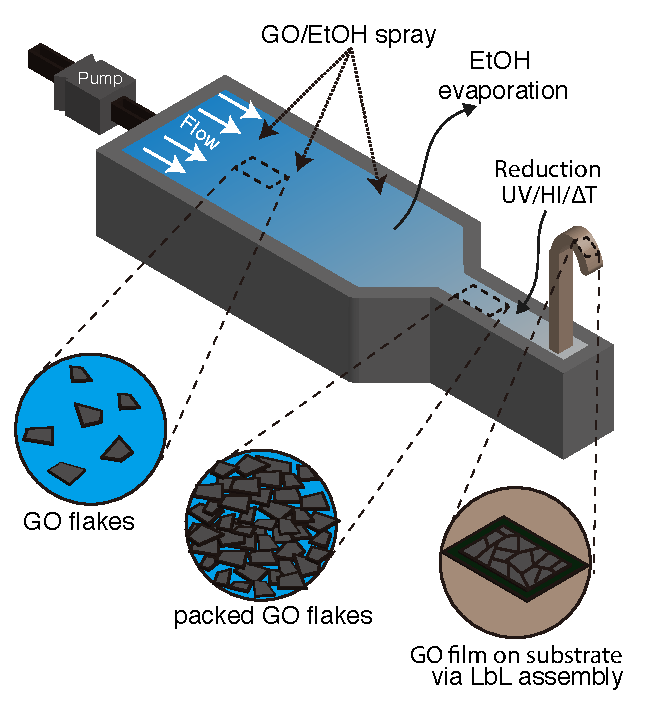
\includegraphics[width=3.5in]{paper2/Fig5.pdf}
  \caption{\textbf{Hybrid casting method}. A GO/ethanol (EtOH) mixture is sprayed on the water surface. A pump ensures the flow of GO flakes, which float at the water/air interface. The GO film at the interface can be packed with the use of movable barriers similar to LB casting. The floating GO layer can then be transferred to a solid substrate via vertical dip-coating. It is possible to insert reduction techniques, such as UV or hydroiodic acid (HI), in the casting method in order to obtain CM-GO.}
  \label{Fig5_pap2}
\end{figure}

\section{Conclusions}
Here, we suggested a GOM categorization method and report four critical challenges that need to be addressed to advance the development of more reliable high-performance GOMs and increase the signal-to-noise ratio in the research field. At the same time, reviewers should be holding authors to accurately perform detailed GO and GO laminate characterization, as well as performance-related permeability/rejection experiments, to ensure that the GO material reported in investigations is in accordance with future standardization. These efforts would guide the GO community toward commercialization for industrial applications and make GO a valid alternative material for membrane technology.